\chapter{数值实验}\label{chp:experiments}
本章我们将提出的新方法运用到Hopkins155~\cite{tron2007benchmark} 和 NUS-WIDE
~\cite{chua2009NUS} 数据集上, 并和SSC、LRR 比较, 说明新算法的优势.

\section{运动分割}
\begin{figure}[hb]
  \centering
  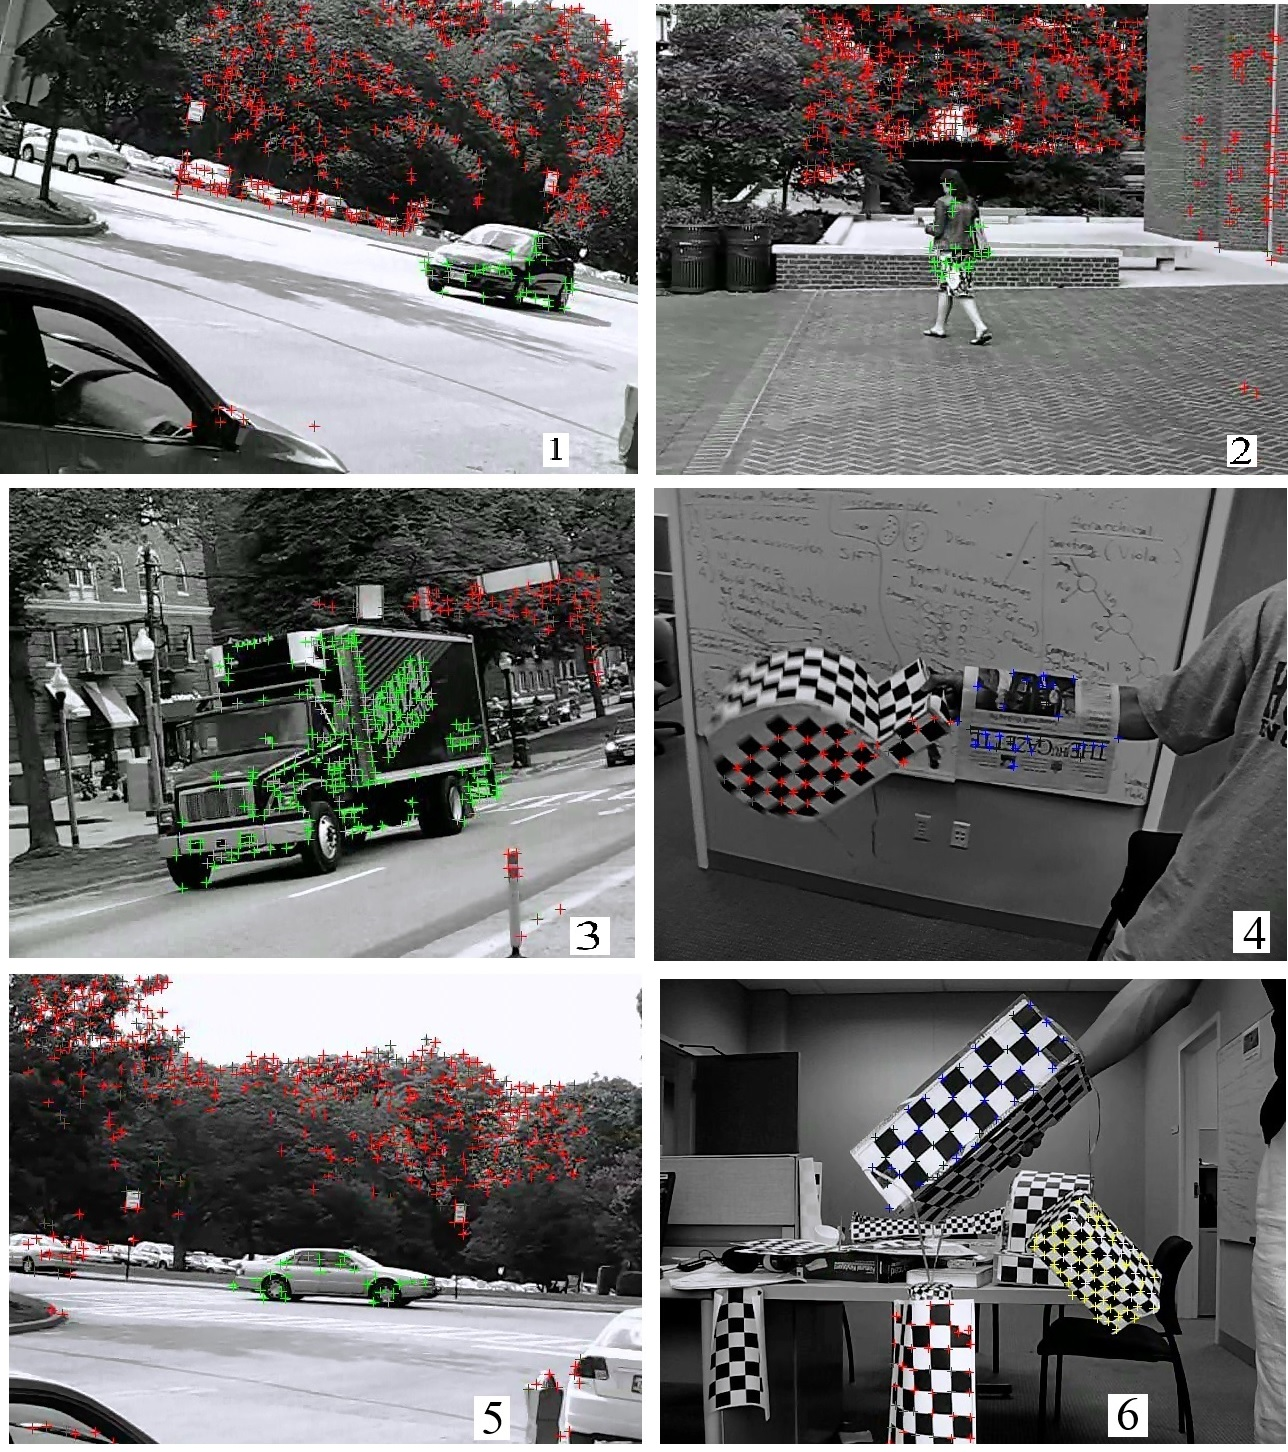
\includegraphics[width=0.7\textwidth]{hopkins}
  \caption{Hopkins155 中的视频某些帧}
  \label{fig:hopkins}
\end{figure}
Hopkins155数据集包含155个视频, 每个视频中有2或3个物体.
主要分成三种类型: 棋盘类, 如\autoref{fig:hopkins} 中4, 6所示,
人们手持棋盘状物体做各种运动, 用相机拍摄视频, 然后将棋盘点在每一帧中
的位置记录下来, 组成高维数据; 交通类, 如\autoref{fig:hopkins} 中1, 3, 5所示,
视频记录了两或三辆车的运动; 其他非刚性运动, 如\autoref{fig:hopkins} 中2所示,
包括人走路, 关节, 头部运动等.

从拍摄图中可以看出, 被跟踪的点来自多个运动实体, 如果把视频看作很多张顺序
图片, 那么每个被跟踪点都有一系列在图片中的相对位置. 我们要根据这些位置,
将每个点分类, 即将来自同一个运动实体的点归为一类.
\begin{table}[!htb]
  \centering
  \begin{tabular}{|c|c|c|c|c|}
	\hline
	算法 & SSC  & LRR  & MT-SSC        & G-SSC         \\ \hline \hline 
	棋盘(78组) &      &      &               &               \\
	平均数     & 2.12 & 2.79 & \textbf{1.83} & 1.91 \\
    中位数     & \textbf{0.51} & 0.72 & 0.57   &\textbf{0.51}  \\ \hline
	交通(31组) &      &      &               &               \\
	平均数     & 0.29 & 0.95 & \textbf{0.15} & 0.35          \\
    中位数     & \textbf{0.00} & \textbf{0.00} & \textbf{0.00}& \textbf{0.00} \\ \hline
	其他(11组) &      &      &               &               \\
    平均数     & \textbf{0.72} & 2.74 & 1.40          & 1.06          \\
    中位数     & \textbf{0.11} & 0.84 &\textbf{0.11} & \textbf{0.11}   \\ \hline
	所有2类数据  &      &      &               &               \\
	平均数     & 1.52 & 2.31 & \textbf{1.36} & 1.43 \\
    中位数     & \textbf{0.12} & 0.84 & \textbf{0.12} & \textbf{0.12}  \\ \hline
  \end{tabular}
  \caption{包含2个物体的数据聚类错误率(越低越好,单位\%)}
  \label{tab:hopkins2}
  \bigskip
  \begin{tabular}{|c|c|c|c|c|}
	\hline
	算法 & SSC  & LRR  & MT-SSC        & G-SSC         \\ \hline \hline
	棋盘(26组) &      &      &               &               \\
	平均数     & 2.97 & 4.47 & \textbf{2.09} & 2.37 \\
    中位数     & \textbf{0.30} & 0.50 & 0.34 & 0.34          \\ \hline
	交通(7组)  &      &      &               &               \\
    平均数     & \textbf{0.58} & 1.05 & 1.51          & 1.51          \\
    中位数     & \textbf{0.00} & 0.02 & \textbf{0.00}& \textbf{0.00}  \\ \hline
	其他(2组)  &      &      &               &               \\
	平均数     & 1.42 & 5.78 & \textbf{0.78} & 1.79          \\
	中位数     & 0.15 & 0.25 & \textbf{0.12} & \textbf{0.12} \\ \hline
	所有3类数据  &      &      &               &               \\
	平均数     & 2.45 & 3.71 & \textbf{1.82} & 2.10 \\
    中位数     & 0.24 & 0.40 & \textbf{0.14}  & 0.16  \\ \hline
  \end{tabular}
  \caption{包含3个物体的数据聚类错误率(越低越好,单位\%)}
  \label{tab:hopkins3}
\end{table}

\begin{figure}[tb]
  \centering
  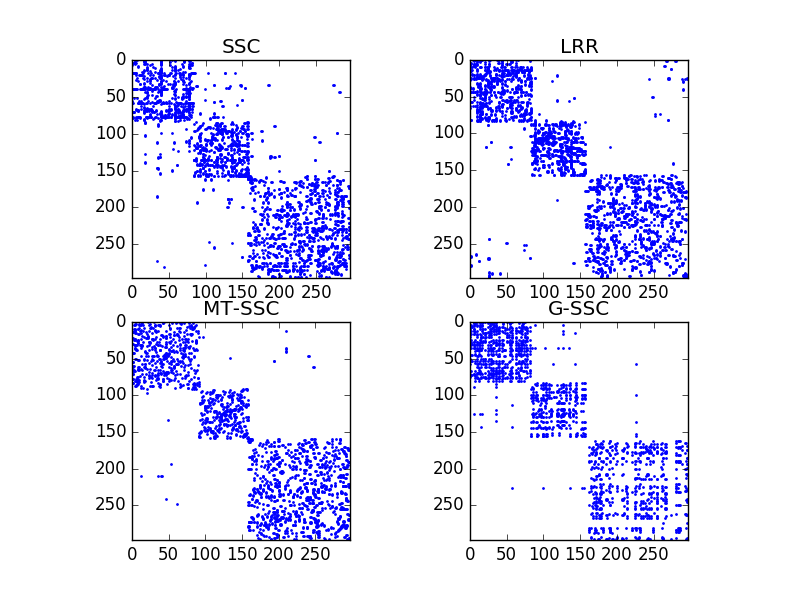
\includegraphics[width=\textwidth]{hopkins_W}
  \caption{SSC, LRR, MT-SSC和G-SSC在cars 10数据上的邻接矩阵}
  \label{fig:hopkins_neig}
\end{figure}
我们比较SSC\footnote{SSC的代码下载自http://vision.jhu.edu/code/.},
LRR\footnote{LRR 的代码下载自https://sites.google.com/site/guangcanliu/.},
MT-SSC,G-SSC四种算法在运动分割上的效果.
由于原始数据点集中在一个相对低维空间中, 导致分组算法很不稳定.
我们用PCA将数据降到\(4L\)维空间 (\(L\)是子空间类数), 并且将之白化(Whitening),
使每个特征有相同的方差. 
取\autoref{alg:nsn} 的参数\(r=2, k=5, \theta=0.05\),
这样得到的分组结果错误率(包含不同类点的分组数/总分组数)为\(0.0063\),
平均每组包含\(4.27\)个点.
进而对原始数据用MT-SSC和G-SSC聚类,
得到聚类错误率(将聚类结果与真实类别比较, 不匹配的点数/总点数)
见\autoref{tab:hopkins2} 和\autoref{tab:hopkins3}. 
可以看出在棋盘类数据中MT-SSC和G-SSC比SSC、LRR表现更优, 也因此总体结果更好.
我们选取一组数据画出了四种算法的邻接矩阵,如\autoref{fig:hopkins_neig} 所示,
相比于SSC,MT-SSC和G-SSC的错误连接更少, 说明其抗干扰能力更强.

\section{图片聚类}
\begin{figure}[htb]
  \centering
  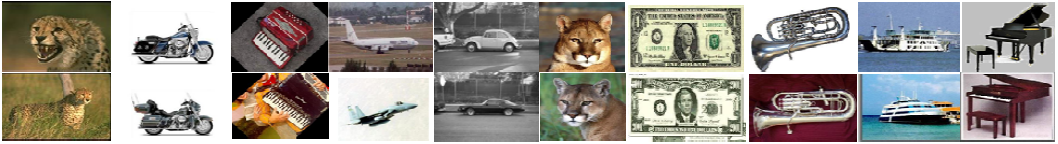
\includegraphics[width=\textwidth]{nusobj}
  \caption{10种物体的图片,这里每样展示了两张}
  \label{fig:nus}
\end{figure}
NUS-WIDE~\cite{chua2009nus} 数据集提供了269648张真实物体
和场景的照片,包括飞机、动物、建筑等等.
我们挑选了其中1000张,他们分别属于10种类别
(如\autoref{fig:nus} 所示有豹子、摩托车、手风琴、飞机等).
NUS-WIDE还提供了每张照片的底层特征,包括64维的LAB空间色彩分布向量,
144维的 HSV 空间色彩相关度向量, 73维的边缘分布向量,
128维的小波纹理, 225维的分块颜色矩(Color Moment)向量以及
500维的SIFT特征向量.在我们的数值例子中,由于时间和存储的限制舍弃了
SIFT 特征, 只用其他634维的特征,这样每张照片都对应634维空间中的一个点.
同时从10种类别中抽3种作为一组, 这样总共有120组测试数据, 每组包含3类300个点.
由于来自同一种物体的图片在色彩、纹理等方面具有很强的相关性, 所以它们近似分布
在一个低维子空间上.

\begin{table}[tb]
  \centering
  \begin{tabular}{|c | c | c | c |}
	\hline
	  算法 & SSC & MT-SSC & G-SSC \\	\hline  \hline
      错误率均值(\%) & 17.80 & 12.51 & \textbf{11.29} \\	\hline
      错误率中位数(\%) & 13.49 & 9.92 & \textbf{8.57} \\	\hline
  \end{tabular}
  \caption{SSC,MT-SSC和G-SSC在NUS-WIDE上的表现}
  \label{tab:nus}
\end{table}
\begin{figure}[t]
  \centering
  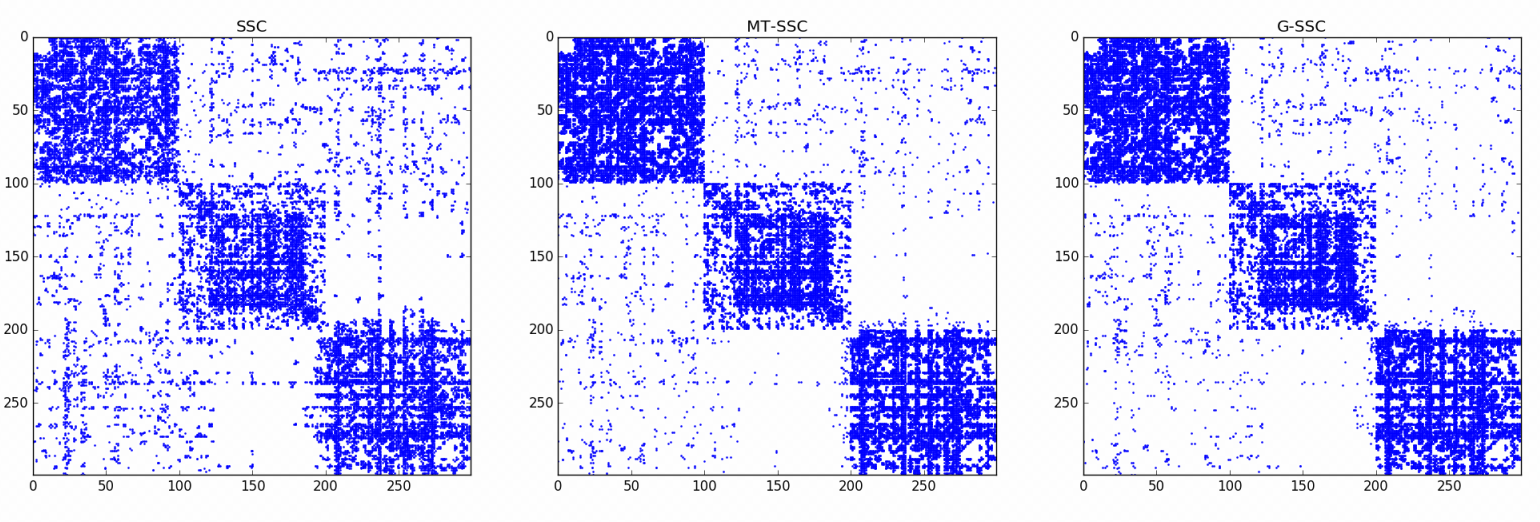
\includegraphics[width=0.8\textwidth]{nus_W}
  \caption{SSC, MT-SSC, G-SSC 在一组测试集上生成的邻接图}
  \label{fig:nus_W}
\end{figure}
\begin{figure}[t!]
  \centering
  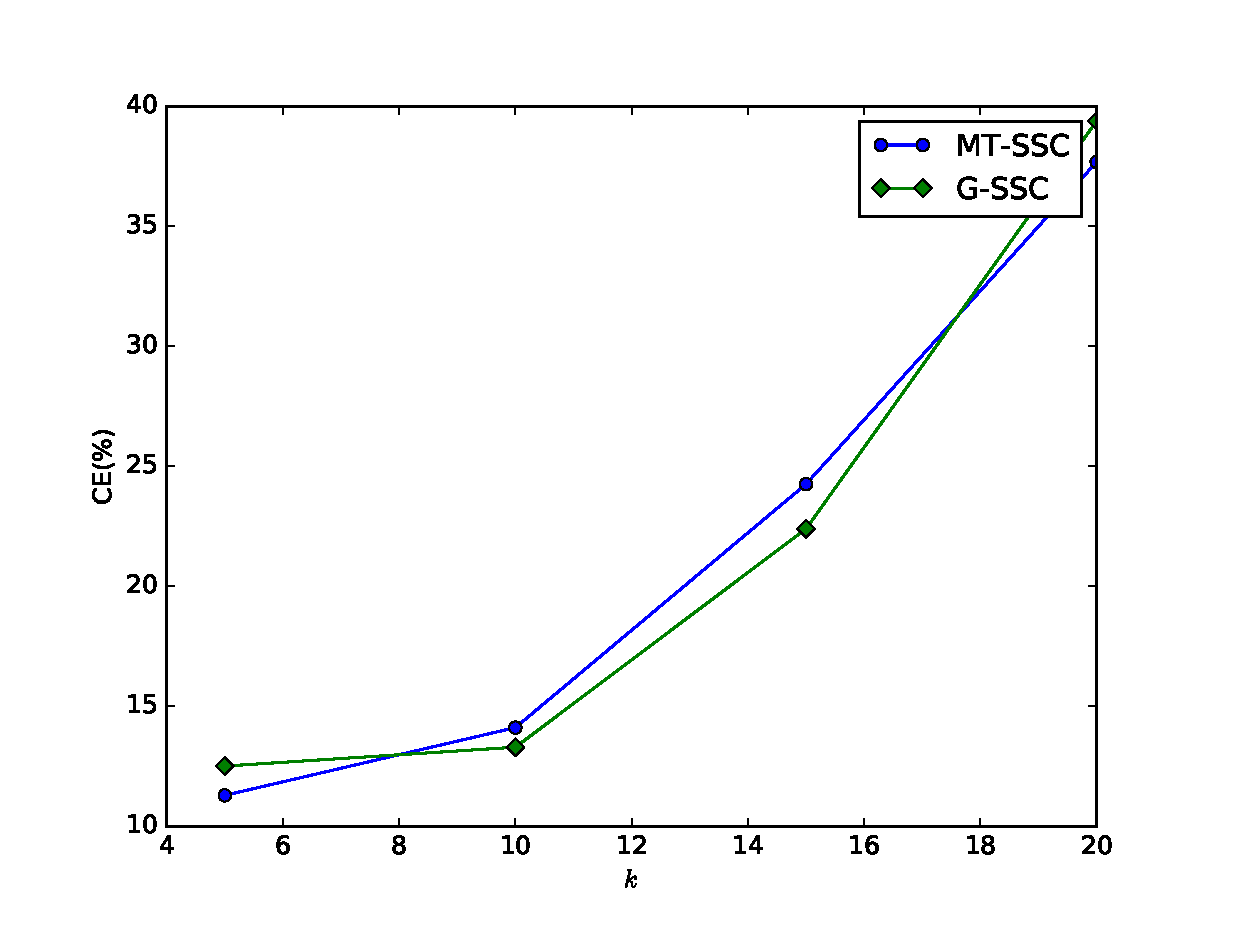
\includegraphics[width=0.6\textwidth]{nus_k}
  \caption{最近邻参数\(k\)对聚类平均错误率的影响}
  \label{fig:nus_k}
\end{figure}
对于分组算法, 同样用PCA将数据降到20维, 并且白化.
取拓展最近邻的参数\(k=5, \theta=0.05, \kappa=0.1\),
得到的分组结果错误率为\(0.0082\), 平均每组包含\(6.42\)个点.
进而对原始数据用MT-SSC和G-SSC算法,
并与SSC比较得到结果如\autoref{tab:nus}.
可以看出MT-SSC、G-SSC 较SSC 聚类正确率更高.
\autoref{fig:nus_W} 是三种算法在某组数据上的邻接图比较,
可以看出MT-SSC和G-SSC比SSC的邻接图错误连接更少,
且同类之间连接更紧密. 我们取了不同的邻居增长参数\(k\)
观察其对聚类结果的影响. 从\autoref{fig:nus_k} 可以看出
最近邻居参数不宜选取的过大, 虽然理论上\autoref{alg:nsn} 
有一定的鲁棒性, 但过大的\(k\)可能会混入很多错误点, 从而
影响阈值\(\theta\)的筛选能力, 并导致自表示发生很大偏差,
降低聚类准确率.

\chapter{总结与展望}
本文介绍了子空间聚类问题, 以及目前公认最有效的方法:
稀疏子空间聚类(SSC)和低秩表示(LRR). 并且列举了基于SSC稀疏自表示思想
的一系列算法. 本文针对SSC的两点不足, 提出了新的多任务和组稀疏子空间聚类方法,
其基本思路是利用数据的局部信息, 将数据点分组. 我们借鉴了~\cite{heckel2013noisy}
中夹角最近邻的想法, 将其推广到投影最近邻, 提出了拓展最近邻算法,
从而将每个点与它在同一局部子空间的点分为一组, 得到指标集族\(\Omega\).
有了分组结果后, 我们提出多任务方法MT-SSC和组稀疏方法G-SSC.
MT-SSC寻求对每个分组内点的同时表示, 而G-SSC将\(\ell_1\)正则化项替换成
\(\ell_{\Omega, 1}\), 以便表示系数相对比较稠密, 从而提升谱聚类的稳定性.

我们对拓展最近邻算法, MT-SSC和G-SSC做了理论分析. 得到在半随机模型下,
如果子空间之间的相关度满足一定条件, 那么拓展最近邻算法第一次循环
加入的点有较大概率和自身在同一子空间. 同时我们还给出了确定性模型下
MT-SSC和G-SSC的表示系数的非零项对应同一子空间中点的条件.
最后我们将新算法在Hopkins155和NUS-WIDE数据集上进行数值实验,
并与SSC、LRR比较. 验证了MT-SSC和G-SSC能在一定的程度上提升聚类结果.

多任务和组稀疏子空间聚类也存在一些问题, 首先分组结果的正确性没有保证,
而如果分组错误, 很可能会对聚类结果带来很大的影响.
其次所需参数过多, 需要给出一些自动选取参数的方法.
最后MT-SSC, G-SSC要求分组互不相交, 然而最近邻集合是有重叠的,
下一步可以考虑利用重叠组稀疏(Overlap Group LASSO)~\cite{jacob2009group},
处理分组有重叠的情形.

另外一个长期困扰自表示类型方法的问题是它们都以观测数据本身作为
字典进行表示, 而观测数据中所含的噪声、缺损、奇异值等都会使字典的
效果下降. 本文作者尝试基于分组结果,用每一组的点得到一个局部的子空间
结构,用每个局部子空间的正交基代替数据本身进行回归表示.如果给定指标集族
\(\Omega=\{\cI_1, \cI_2, \ldots, \cI_{|\Omega|}\}\),
对\(\cI_j\)我们用\(X_{\cI_j}\)的前\(r\)个左奇异向量组成矩阵\(U^{(j)}\)代替\(X_{\cI_j}\).
假设\(i \in \cI_1\), 那么将G-SSC的优化问题换成
\begin{equation}
  \min_{c} \, \|\reshape(c)\|_{2, 1}+\frac{\lambda}{2}
  \left\|x_i-\left[ U^{(2)} U^{(3)} \cdots U^{(|\Omega|)}\right]c\right\|_2^2.
  \label{eq:ussc}
\end{equation}
其中\(\reshape(c)\)是将向量\(c\)的元素\(r\)个一列排成矩阵.
这样字典不再是原始数据而是每类点张成空间的基,在一定程度上可以
使字典更稳定,减少噪音干扰. 不过在Hopkins155 数据集上, \eqref{eq:ussc} 表现不佳,
这可能来由于噪音干扰使得\(U^{(j)}\)中包含了不在自身子空间中方向,
具体原因和改进方法值得进一步探索.
